\chapterimage{unidades/2_informacion/1_bajo_nivel/imagenes/cover}
\chapterimagedescription{Fotografía artistica que representa información}
\chapterimageauthor{Fotografía de Pixabay}

\chapter{Bajo nivel}

\setcounter{section}{2}
\section{Actividades}

\begin{exercise}
Dada la imágen a continuación, expresela como un único
número utilizando la misma codificación que se aplicó
en este capítulo.

\centerline{
\includegraphics[scale=0.5]{unidades/2_informacion/1_bajo_nivel/imagenes/pixels_smile.png}}
\end{exercise}

En primer lugar, utilizamos la tabla de colores para marcar cada celda con el
número correspondiente. También marcamos el ancho y el alto de la imágen.

\centerline{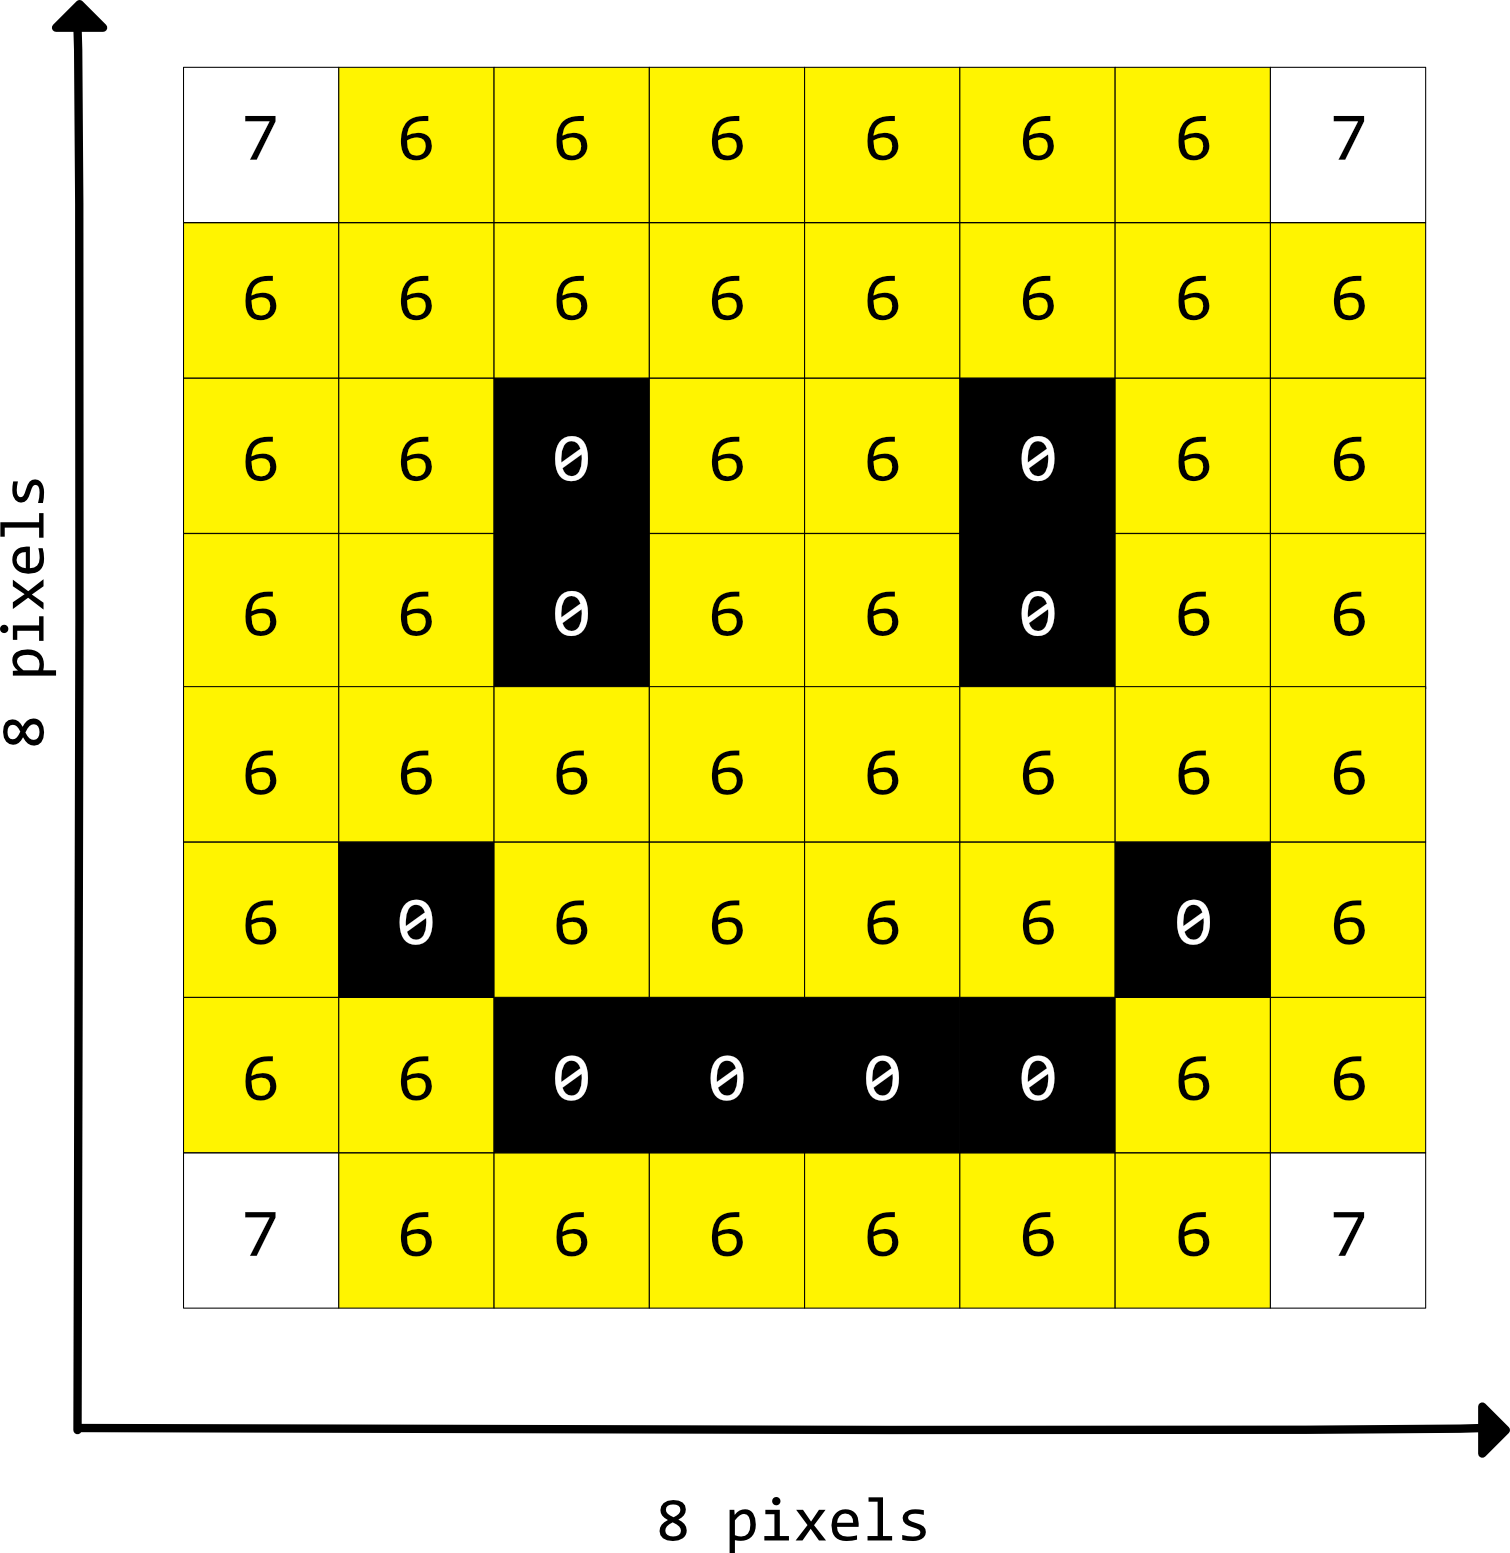
\includegraphics[scale=0.5]{soluciones/2_informacion/1_bajo_nivel/imagenes/pixels_smile_labeled.png}}

Ahora podemos eliminar la imágen y quedarnos solo con los números.

\centerline{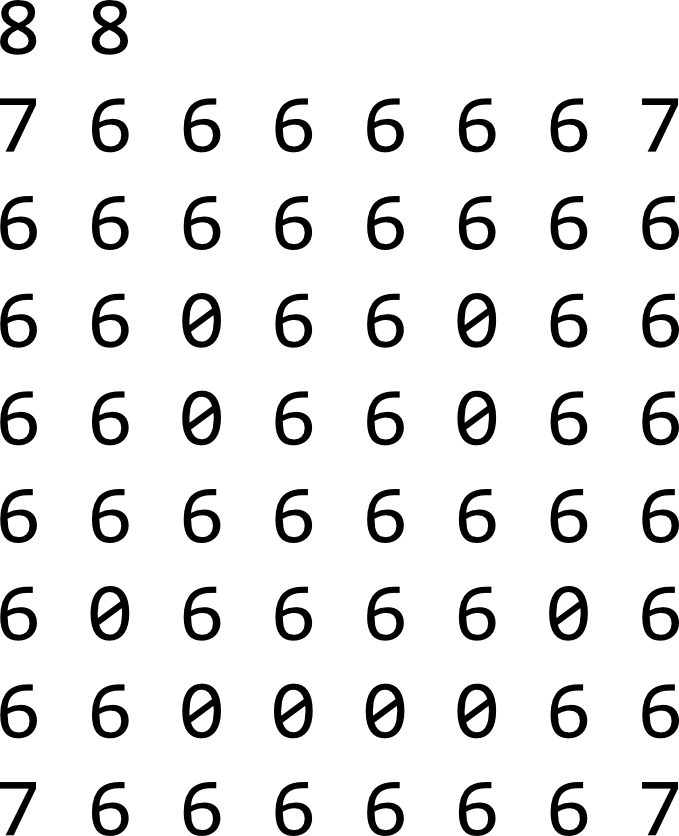
\includegraphics[scale=0.5]{soluciones/2_informacion/1_bajo_nivel/imagenes/pixels_smile_numbers.png}}

Y ahora, podemos eliminar el formato para obtener el número que representa dicha imágen.

\vspace{0.3cm}
\centerline{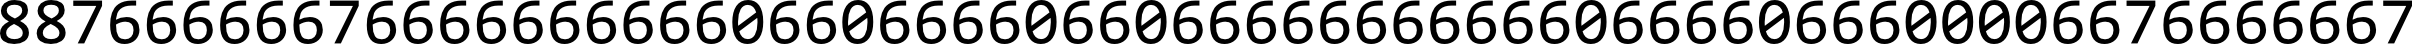
\includegraphics[scale=0.65]{soluciones/2_informacion/1_bajo_nivel/imagenes/pixels_smile_code.png}}
\vspace{1cm}

\begin{exercise}
La tabla mostrada en este capítulo para representar letras como números
corresponde a la codificación ASCII. Utilizando esa tabla se pide que codifique
la siguiente frase como una serie de números.

\textbf{SOMOS LO QUE PROGRAMAMOS}
\end{exercise}

El texto se corresponde con el siguiente código:

\textbf{83 79 77 79 83 32 76 79 32 81 85 69 32 80 82 79 71 82 65 77 65 77 79 83}
\vspace{1cm}

\begin{exercise}
Nuevamente, usando ASCII, se pide ahora que decodifique el siguiente mensaje
expresado como una serie de números.

\textbf{80 82 79 71 82 65 77 79 32 76 85 69 71 79 32 69 88 73 83 84 79}
\vspace{1cm}

\end{exercise}

El código debería leer:

\textbf{PROGRAMO LUEGO EXISTO}
\vspace{1cm}

\begin{exercise}
Si contamos con una computadora con 16 cables para representar nuestros datos,
¿Qué cantidad de números distintos pueden representarse con ellos?
\end{exercise}

Si orestaron atención, cada cable nos permite 2 opciones, con electricidad, o
sin ella. Si solo tengo un cable, tengo 2 números posibles. Si tengo 2 cables,
puedo tener 4 números posibles representados de diferentes formas (ámbos cables
sin electricidad, ámbos con electricidad, el primero con electricidad y el
segundo sin, y finalmente el primero sin y el segundo con electricidad).

Así, se obtiene que la cantidad de números posibles depende de la cantidad de
cables, siendo equivalente a:

\begin{equation}
    2^{\text{cant. cables}} = \text{cant. números distintos}
\end{equation}

En este caso, con 16 cables, tenemos:

\begin{equation}
    2^16 = 65536
\end{equation}

Es decir, \textbf{hay 65536 números distintos que pueden ser representados}.
\vspace{1cm}

\begin{exercise}
Un chiste de informáticos reza lo siguiente:

\textbf{``Solo hay 10 tipos de personas en este mundo, los que entienden binario
y los que no''}

En qué radica la gracia del chiste.
\end{exercise}

Una códificación clásica para números utilizando binario (con dos bits)
representa a los números de la siguiente forma:

\vspace{0.3cm}
\begin{tabular}{c | c}
    Número & Binario \\
    \hline
    0 & 00 \\
    1 & 01 \\
    2 & 10 \\
    3 & 11 \\
\end{tabular}
\vspace{0.3cm}

Así, 10 en binario, es 2. El chiste reza entonces que hay solo dos tipos de
personas en el mundo, aquellos que entienden binario, y aquellos que no, pero
emplea binario para decirlo, haciendo que solo uno de esos dos grupos pueda
comprender el chiste.
